\documentclass{article}[11pt]
\textheight 8.5in
\usepackage{graphicx}
\usepackage{float}%for forcing position of figs
\usepackage{hyperref}
\usepackage{amsmath}
\usepackage{amssymb}

\begin{document}
\begin{center}
Siddharthan Rajasekaran\\

\end{center}

\section{Summary of Discussions}
In this report, we will show the results of Advantage-Actor Critic (a2c) on a pendulum swing up task. 

\section{Environment}
Observation: ($\cos\theta$, $\sin\theta$, $\dot\theta$)\\
Reward: $-(\theta^2 + 0.1\dot\theta^2 + 0.001u^2)$\\

The goal is to balance the pendulum at the vertical position at zero velocity with minimal effort. Further, we will discuss in future the convergence with and without the Value function initialization. 

\section{Results}

Results of implementation of Advantage Actor Critic. Quantities being compared
\begin{itemize}
\item Average reward (EpRewMean): The average reward per episode in the current iteration. We perform roll outs 10 times each iteration to get a Monte-Carlo estimate of returns. EpRewMean is the average over these roll outs
\item KL divergence (KLOldNew): The KL divergence between the old policy (of the previous iteration) and the new policy. A huge spike means we are taking a large step in policy update and want to make the step size smaller
\item Entropy: The entropy of the current stochastic policy. A very low value means that we are not exploring enough.
\item Explained Variance (EVBefore): This is the explained variance of the current fit of the value function and is a metric generally used to see the performance of regression. 
Mathematically, Explained variance = $\frac{\text{Residue Variance}}{\text{Total Variance}} = \frac{Var(\hat{y} - y)}{Var(y)}$, where $\hat{y}$ is the estimate of the value from our current approximation and y is the return computed empirically by rolling out the system. This is the proportion of variance of data that we explain. 

A value close to zero would mean we are doing worse than the mean estimate. A sudden increase in the explained variance would mean we are over-fitting. 

\end{itemize}

 \begin{figure}[H]
  \begin{center}
    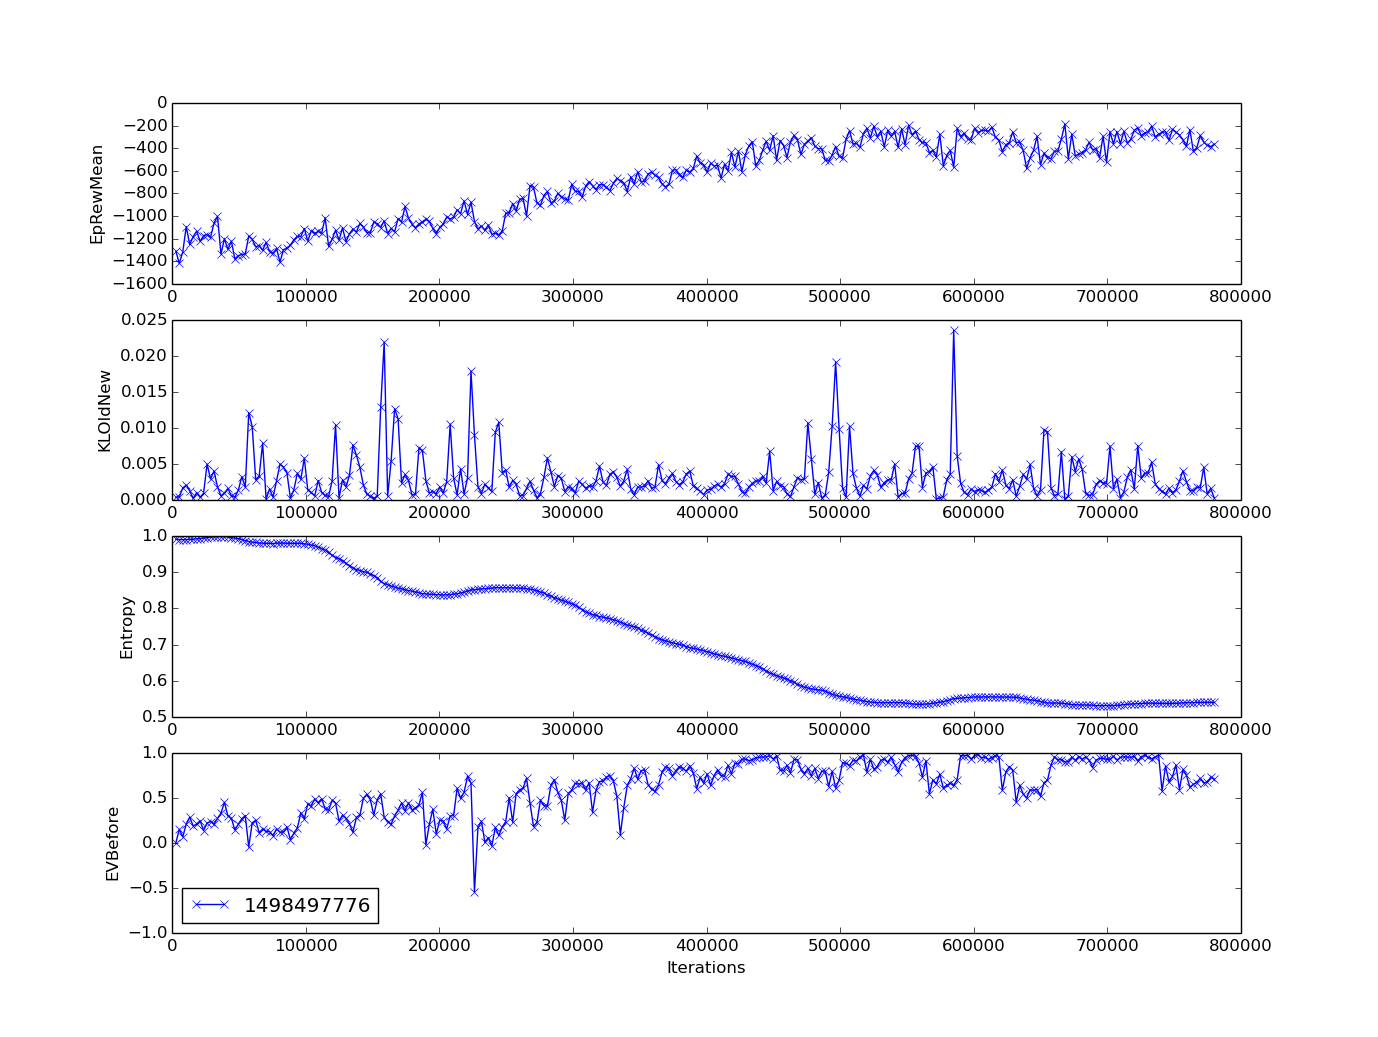
\includegraphics[width=1.4\linewidth]{images/plot}
    \caption{ Results of a2c with quadratic basis approximation for value function and neural net approximation for policy.}
    \label{fig:5grid}
  \end{center}
\end{figure}



\bibliographystyle{plain}
\bibliography{bibfile}
\end{document}
